\documentclass[letterpaper,11pt]{article}

\usepackage[margin=1in]{geometry}
\usepackage{fontspec}
\setmainfont{Times New Roman}
\usepackage[protrusion=true, final]{microtype}
\RequirePackage{graphicx}
\usepackage{caption}
\usepackage{float}
\usepackage{enumitem}
\usepackage{siunitx}
\usepackage{amsmath}
\usepackage[table]{xcolor}
\usepackage[style=numeric-comp, maxnames=99, minnames=1, sorting=none]{biblatex}
\addbibresource{citations.bib}
\usepackage[colorlinks = true,
linkcolor = blue,
urlcolor  = blue,
citecolor = blue,
anchorcolor = blue,
pdftitle={Exercise - Passivelogic},
pdfauthor={Remi Patureau}]{hyperref}
\usepackage[capitalize]{cleveref}

\title{Technical Case Study}
\author{Rémi Patureau}
\date{}


\begin{document}
	
	\maketitle
	
	\section{Part A — Digital Twin (Core Physics)}
	
	\subsection{Task 1 — Thermal Model}
	
	\subsubsection{Statement}
	
	Build a physics-based thermal model of NovaCool. Your model should capture heat generation
	from servers, airflow between hot and cold aisles, and the cooling effect of the CRAH units. A
	lumped-parameter or reduced-order approach is preferred over CFD — we value clarity and speed
	over spatial resolution.
	\begin{itemize}[label=--]
	\item Model each rack as a heat source whose power draw varies with a provided workload trace
	(CSV attached below).
	\item Implement a simplified airflow model: cold air enters the cold aisle at a CRAH supply
	temperature, absorbs heat as it passes through racks, and exits into the hot aisle.
	\item Model CRAH behavior: each unit removes heat from the return air using a chilled-water loop
	with a configurable flow rate and supply temperature.
	\item Simulate at 1-minute time steps over a 24-hour period.
	\item Produce time-series plots of: (a) average cold-aisle temperature, (b) average hot-aisle
	temperature, (c) peak rack outlet temperature, and (d) total cooling power consumed.
	\end{itemize}

	\subsubsection{Solution}
	
	Different levels of approximation are possible. As a first approach, I consider that there is no thermal mass, as the inertia is very low (around 2 minutes). Two elements are modeled, the racks and the exchange with the water loop. To do so, I considered a constant efficciency ot the heat exchanger, and therefore considered the CRAH as a heat exchanger, with $\varepsilon = 0.7$.
	
	To my understanding, the controls for the temperature are not provided, only some requirements regarding the water loop.
	
	The elements are modeled as follows:
		
	\begin{equation}
		P_{rack} = \dot{Q}_{air} = \dot{m}_{air} \, Cp_{air} \, \Delta T
	\end{equation}
	
	\begin{equation}
		C_{min}= \min{(\dot{m}_{air} \, {Cp}_{air} \ ,\ \dot{m}_{water} \times {Cp}_{water})}
	\end{equation}
	
	\begin{equation}
		\dot{Q}_{air}  = \dot{Q}_{water} = \varepsilon \, Cmin \, (T_{in, air} - T_{in, water})
	\end{equation}
	
	\begin{equation}
		\label{eq:cst_tc}
		T_{out, air} = T_{in, air} - \dfrac{\dot{Q}_{air}}{\dot{m}_c \, Cp_{air}}
	\end{equation}
	
	\begin{equation}
		\label{eq:cst_tf}
		T_{out, water} = \dfrac{\dot{Q}_{water}}{\dot{m}_{water} \, Cp_{water}} + T_{in, water}
	\end{equation}
	
\begin{figure}[H]
	\centering
	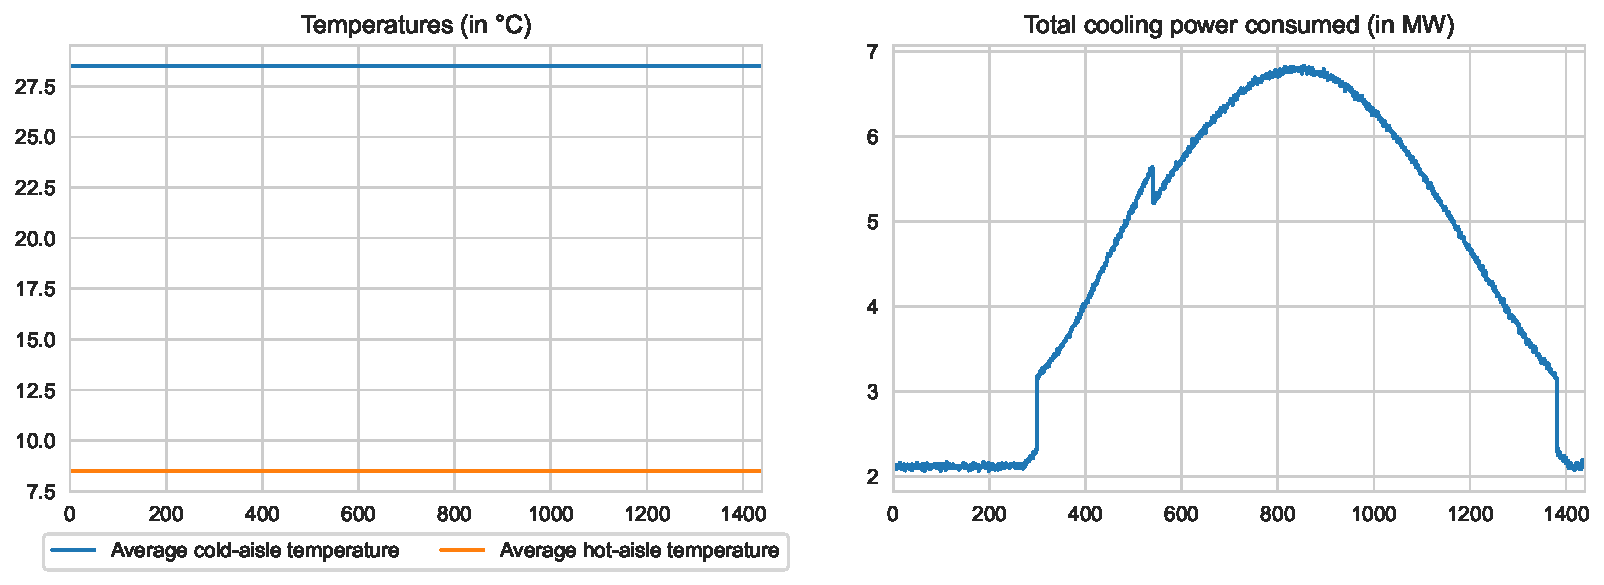
\includegraphics[width=\textwidth]{plots/task1}
	\caption{Test}
	\label{fig:task1}
\end{figure}

With more time, two improvements in the modeling are possible:
\begin{itemize}
	\item 
\end{itemize}
	
\subsection{Task 2 — Power \& System Coupling}

Extend your simulation to model the electrical power path and its coupling with thermal dynamics.
\begin{itemize}[label=--]
	\item Model UPS efficiency as a function of load (quadratic curve; efficiency peaks around 50–75\% load).
	\item Include cooling infrastructure power: CRAH fans and chilled-water pumps should consume
	energy proportional to thermal load.
	\item Compute Power Usage Effectiveness (PUE) = Total Facility Power / IT Load as a time-varying
	metric.
	\item Show how PUE varies over the 24-hour period as workload and ambient conditions change.
\end{itemize}

\subsection{UPS efficiency (quadratic curve)}

\begin{equation}
\eta(x) = \eta_{peak} - k \, (x - x_{peak})^2
\end{equation}

With defaults $\eta_{peak} = 0.965$ (96.5\% peak efficiency), $x_{peak} = 0.65$ (peak at 65\% load), and k = 0.20. This means the UPS is most efficient at around 50–75\% load and wastes more power at very low or very high loads. 

\subsection{Fan power}

\begin{equation}
P_{fan} = P_{nomina}l \, speed^3
\end{equation}



\textbf{Pump power}: Scales linearly with cooling duty (fraction of zone capacity being used), with a 15% idle floor representing minimum circulation.

\textbf{Chiller power}: Computed via a Coefficient of Performance (COP) model:

\begin{equation}
P_{chiller} = \frac{Q_{cooling}}{COP}
\end{equation}

Here the COP is considered constant for this example. It should be approximated in a better way, for example via the empirical MDOE2 method.

\subsection{PUE}

\begin{equation}
PUE = (P_UPS_input + P_{fans} + P_{pumps} + P_{chiller} + P_{other}) / P_IT
\end{equation}

A small overhead (1\% of capacity) covers lights, security, and networking.

\begin{figure}[H]
	\centering
	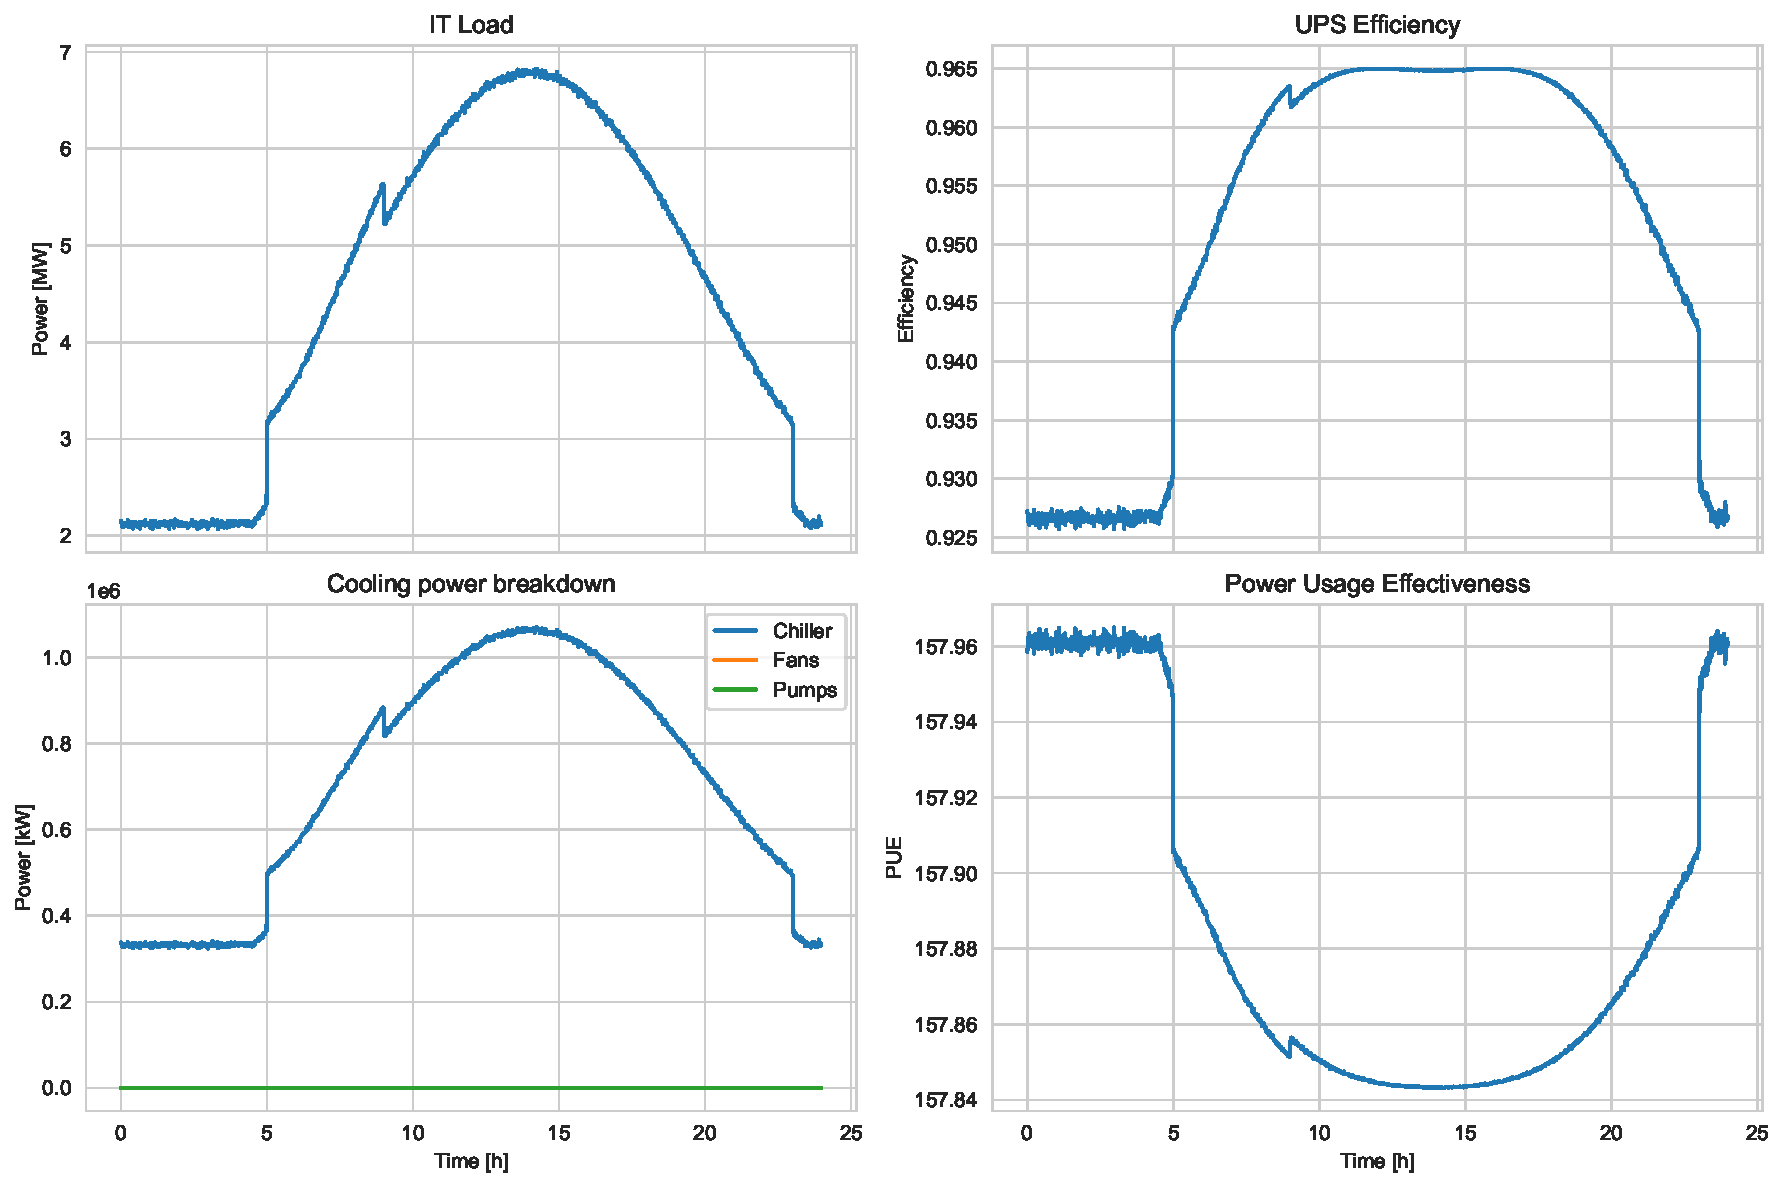
\includegraphics[width=\textwidth]{plots/task2}
	\caption{Thermal Model}
	\label{fig:task2}
\end{figure}


\subsection{Task 3 — Model Validation \& Calibration}
We provide a reference dataset (synthetic) representing 24 hours of sensor readings from
NovaCool. Compare your simulation outputs against this reference.
\begin{itemize}[label=--]
	\item Compute error metrics: RMSE, MAE, and max absolute error for temperature predictions.
	\item Identify time intervals where your model diverges most from the reference data and
	hypothesize why.
	\item Describe at least two concrete approaches you would use to calibrate or improve model
	fidelity (e.g., parameter tuning, data assimilation, Bayesian calibration).
\end{itemize}

\begin{figure}[H]
	\centering
	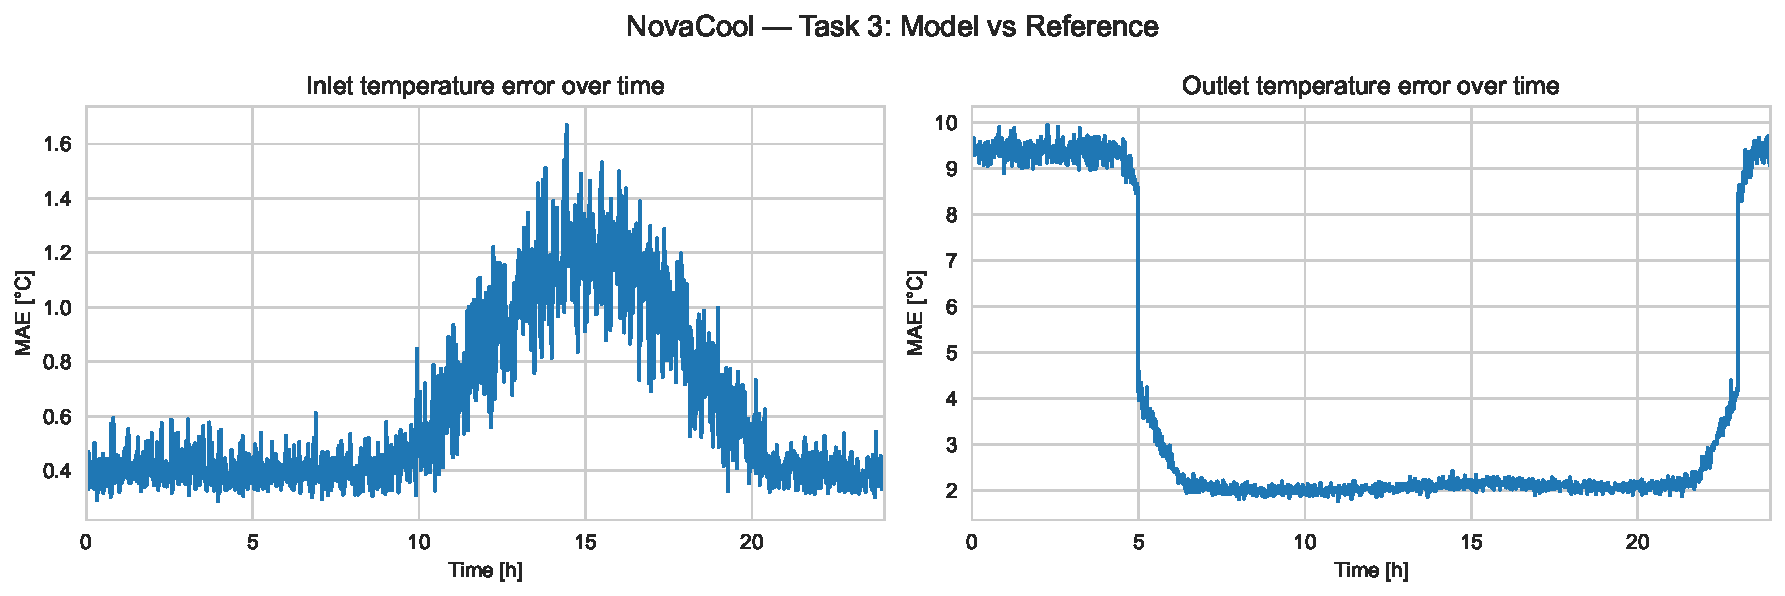
\includegraphics[width=\textwidth]{plots/task3}
	\caption{Temperature differences over 24h}
	\label{fig:task3}
\end{figure}

Inlet  — RMSE: 0.78 °C  MAE: 0.62 °C  MaxAE: 3.36 °C\\
Outlet — RMSE: 5.31 °C  MAE: 4.00 °C  MaxAE: 16.35 °C

Comparing the mass flow rate, we obtain similar results:

\begin{figure}[H]
	\centering
	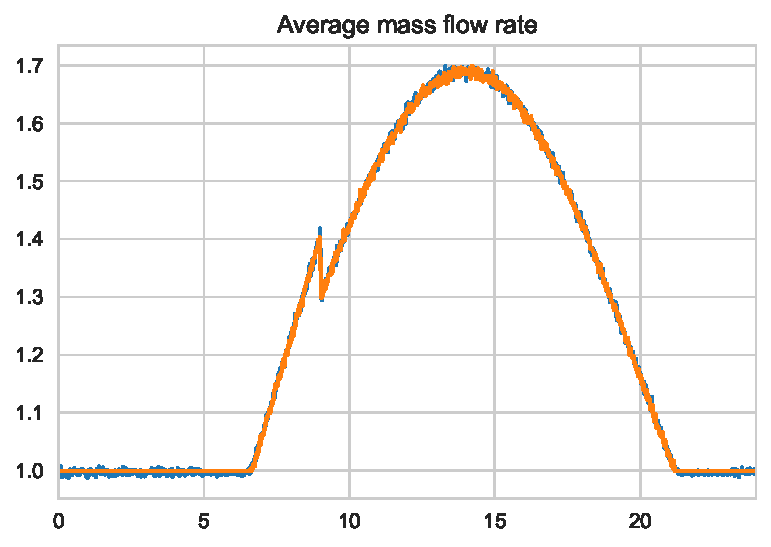
\includegraphics[width=0.7\textwidth]{plots/avgmf}
	\caption{Mass flow rate difference over 24h}
	\label{fig:avgmf}
\end{figure}

\begin{figure}[H]
	\centering
	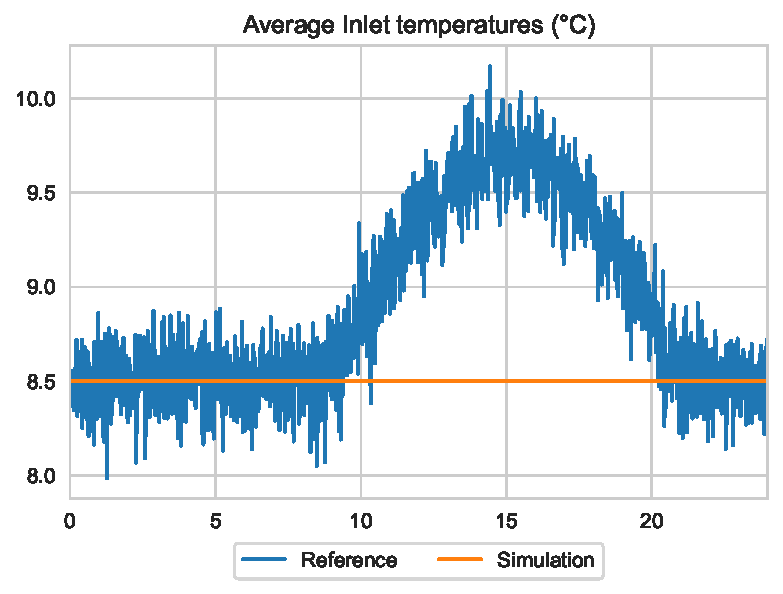
\includegraphics[width=0.7\textwidth]{plots/avgin}
	\caption{Inlet reference and simulated temperatures over 24h}
	\label{fig:avgin}
\end{figure}

\begin{figure}[H]
	\centering
	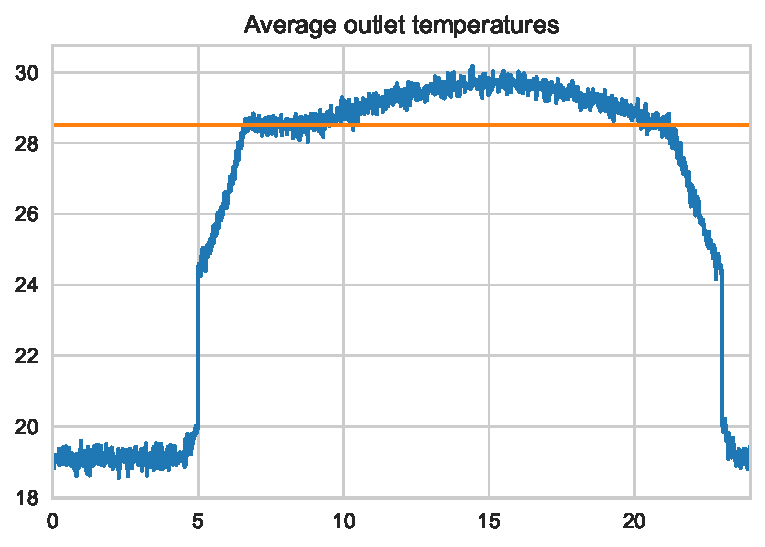
\includegraphics[width=0.7\textwidth]{plots/avgout}
	\caption{Outlet reference and simulated temperatures over 24h}
	\label{fig:avgout}
\end{figure}

\section{Part B — Control \& Environment Design}

\subsection{Task 4 — Control Policy}
Define and implement a simple control policy for the NovaCool facility. The goal is to maximize
compute throughput (i.e., allow racks to run at higher utilization) while respecting thermal safety
constraints.

\textbf{Objective \& Constraints}
\begin{itemize}[label=--]
	\item Maximize total IT load served across all racks over the 24-hour window.
	\item Hard constraint: No rack outlet temperature may exceed \qty{40}{\celsius} at any time step.
	\item Soft constraint: Minimize total cooling energy consumed (PUE should improve, not
	degrade).
\end{itemize}

\textbf{Available Control Inputs (choose a subset)}
\begin{itemize}[label=--]
	\item CRAH supply temperature setpoint (per unit)
	\item CRAH fan speed / airflow rate (per unit)
	\item Workload redistribution across racks (optional stretch goal)
\end{itemize}

\textbf{Deliverables}
\begin{itemize}[label=--]
	\item Describe your control policy (heuristic, PID, rule-based optimizer, or other approach).
	\item Run your policy on the 24-hour workload trace and compare results against a no-control
	baseline (fixed CRAH setpoints).
	\item Report: (a) total IT load served, (b) number of thermal violations, (c) total cooling energy, and
	(d) PUE improvement.
\end{itemize}

\subsection{Task 5 — RL-Ready Environment Interface}
Imagine a team of RL engineers wants to train autonomous control agents using your simulator.
Wrap your digital twin as a reusable environment with a clean API. You do not need to train an RL
agent — focus on the environment design.

\textbf{Required Interface}

Implement a minimal Gym-style interface


Define clearly:
\begin{itemize}[label=--]
	\item Observation space (st): What does the agent see? (e.g., temperatures, loads, ambient
	conditions, time of day)
	\item Action space (at): What can the agent control? (e.g., CRAH setpoints, fan speeds)
	\item Reward signal (rt): How is success measured? (e.g., throughput bonus minus
	thermal-violation penalty minus energy cost)
	\item Episode termination: When does an episode end? (e.g., end of 24h window, or early on
	critical violation)
\end{itemize}
In your write-up, justify your design choices — especially the reward function. Discuss trade-offs between reward
shaping complexity and learning stability.

\section{Part C — Architecture \& Scaling (Discussion)}
Address the following in your write-up and live presentation. No additional code is required for this
section.
\begin{itemize}[label=--]
\item \textbf{Modularity}: How do you structure the codebase so that new subsystems (e.g., a humidity
model, battery storage, or a new cooling technology) can be added without rewriting existing
modules?
\item \textbf{Scaling}: What strategies would you use to run the simulation for a facility 10x larger (2,000
racks) and still complete a 24-hour sim run in under 5 minutes?
\item \textbf{Online correction}: How would you integrate real-time sensor data into a running simulation
to correct model drift (i.e., sim-to-real alignment)?
\item \textbf{Testing}: Describe a testing strategy to ensure simulation correctness as the codebase
evolves.
\item \textbf{Sim-to-real gap}: What are the most likely sources of discrepancy between your simulation
and a real facility, and how would you systematically reduce them?
\end{itemize}

\subsection{Stretch Goals (Optional — for differentiation)}
These are not required, but will be positively noted:
\begin{itemize}[label=--]
	\item Inject a perturbation (e.g., one CRAH fails for 30 minutes) and show how your control policy
	responds.
	\item Compare multiple control strategies (e.g., heuristic vs. PID vs. simple optimizer).
	\item Add stochasticity to the simulation (sensor noise, workload bursts).
	\item Discuss domain randomization or partial observability in the context of your environment
	design.
\end{itemize}

\end{document}